\documentclass[11pt]{article}

\usepackage[margin=1in]{geometry}
\usepackage{amsmath,amssymb,amsthm,mathtools}
\usepackage{booktabs}
\usepackage{enumitem}
\usepackage{array}
\usepackage{tikz}
\usetikzlibrary{positioning,arrows.meta}
\usepackage[hidelinks]{hyperref}
\usepackage{microtype}

\newtheorem{theorem}{Theorem}[section]
\newtheorem{proposition}[theorem]{Proposition}
\newtheorem{lemma}[theorem]{Lemma}
\newtheorem{corollary}[theorem]{Corollary}
\theoremstyle{definition}
\newtheorem{definition}[theorem]{Definition}
\newtheorem{example}[theorem]{Example}
\theoremstyle{remark}
\newtheorem{remark}[theorem]{Remark}

\newcommand{\F}{\mathbb{F}}
\newcommand{\Z}{\mathbb{Z}}
\newcommand{\wt}{\operatorname{wt}}
\newcommand{\nl}{\operatorname{nl}}
\newcommand{\supp}{\operatorname{supp}}
\newcommand{\rank}{\operatorname{rank}}
\newcommand{\ind}{\mathbf{1}}
\newcommand{\lo}{\mathrm{lo}}
\newcommand{\hi}{\mathrm{hi}}
\newcommand{\code}[1]{\texttt{#1}}
\DeclareRobustCommand{\_}{\textunderscore\allowbreak}
\newcommand{\main}{\cite{Main}}

\newenvironment{keyidea}{\begin{quote}\small\textbf{Key idea.}\ }{\end{quote}}

\title{How the Proof Works:\\
A Guided Tour of the Balanced Nonlinearity-$242$ Exclusion}
\author{Daniel Ayomide Shittu}
\date{Companion to \emph{No Balanced $9$-Variable Boolean Function Has Nonlinearity $242$}\\[2pt] \today}

\begin{document}
\maketitle

\begin{abstract}
This companion explains how the master theorem reduces the exclusion of balanced nine-variable functions of nonlinearity $242$ to a finite set of cases, giving $\nl_{\mathrm{bal}}(9)=240$ (with the full $t=100$ rank-$6$ reductions and audited verifiers written out in \code{t100.tex}). It proves nothing new. It follows one thread. A few parity facts about the Walsh spectrum force a single quadratic form on $\F_2^8$ to control the whole function, and one energy identity then turns the problem into a finite list of cases. We explain the handful of tools used on those cases, give a map of where each case is closed, and work one case, agreement counts $114$ and $116$, from start to finish. Every claim points to the place in the main paper~\main{} or in the replay packets where it is proved or checked.
\end{abstract}

\tableofcontents

% ===========================================================================
\section{What is being proved}
% ===========================================================================

Let $F:\F_2^9\to\F_2$. Its \emph{Walsh transform} is
\[
  W_F(\omega)=\sum_{x\in\F_2^9}(-1)^{F(x)+\omega\cdot x},\qquad \omega\in\F_2^9 .
\]
$W_F(\omega)$ measures how well $F$ agrees with the linear function $x\mapsto\omega\cdot x$: it is $512-2d$, where $d$ is the number of disagreements. The \emph{nonlinearity} is the distance from $F$ to the nearest affine function,
\[
  \nl(F)=256-\tfrac12\max_\omega|W_F(\omega)| .
\]
So nonlinearity $242$ means $\max_\omega |W_F(\omega)|\le 28$. $F$ is \emph{balanced} when it takes each value $256$ times, that is, when $W_F(0)=0$.

\paragraph{How flat is that?} Parseval's identity says $\sum_\omega W_F(\omega)^2=2^{18}$ for every $F$. Spread evenly over $512$ frequencies, that is an average square of $512$, a typical size of about $22.6$. A peak of $28$ therefore means the spectrum is almost perfectly flat. Perfect flatness (bent functions) is impossible in an odd number of variables, so $242$ asks for nearly the best possible.

\paragraph{History.} Splicing two bent functions on eight variables gives balanced $9$-variable functions with peak $32$, that is nonlinearity $240$. In 2006--2007 Kavut, Maitra and Y\"ucel found $9$-variable functions with peak $28$ (nonlinearity $242$)~\cite{KMY2006,KMY2007}, but all of them are unbalanced. Nobody found a balanced one, and nobody proved there is none. Brute force is hopeless: there are $\binom{512}{256}\approx 4.7\times10^{152}$ balanced functions. In smaller odd dimensions ($n=1,3,5,7$) the balanced and unrestricted maxima are equal~\main, so $n=9$ is the first place the question has teeth.

\begin{theorem}[Main theorem of~\main]
No balanced $F:\F_2^9\to\F_2$ has $\max_\omega|W_F(\omega)|\le 28$. Hence the largest nonlinearity of a balanced $9$-variable function is $240$, and $n=9$ is the first odd dimension where balance costs nonlinearity.
\end{theorem}

\paragraph{The strategy in one paragraph.} Assume such an $F$ exists. Parity forces a canonical direction $s\in\F_2^9$ (Section~\ref{sec:parity}). Cutting the cube along $s$ gives two $8$-variable halves, and their agreement count $t$ becomes the main parameter (Section~\ref{sec:split}). A $2$-adic ``digit principle'' then shows that one quadratic form on $\F_2^8$ governs both halves (Section~\ref{sec:quadratic}). Parseval turns that into an exact budget, which leaves finitely many cases for each $t$ (Section~\ref{sec:budget}). Each case is closed with a small toolkit (Section~\ref{sec:toolkit}); Section~\ref{sec:map} says which tool closes which case, and Section~\ref{sec:endpoint} works one case in full.

\begin{figure}[ht]
\centering
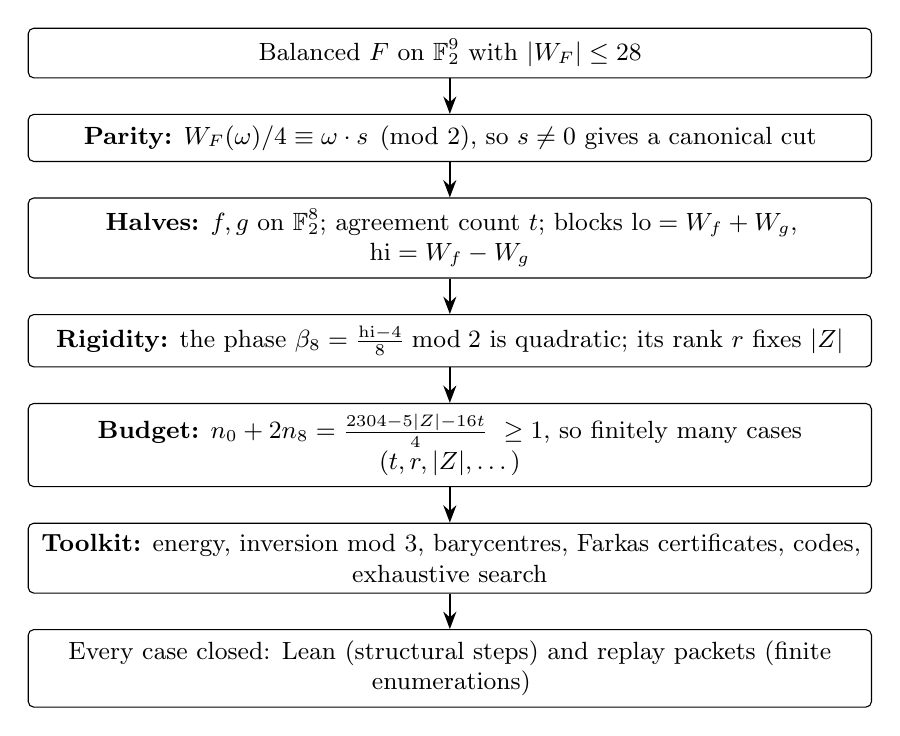
\begin{tikzpicture}[
  box/.style={draw, rounded corners=2pt, align=flush center, font=\small, inner sep=4pt, text width=0.86\textwidth},
  arr/.style={-{Stealth[length=2.2mm]}, thick},
  node distance=4.5mm]
\node[box] (a) {Balanced $F$ on $\F_2^9$ with $|W_F|\le 28$};
\node[box, below=of a] (b) {\textbf{Parity:} $W_F(\omega)/4\equiv \omega\cdot s \pmod 2$, so $s\neq 0$ gives a canonical cut};
\node[box, below=of b] (c) {\textbf{Halves:} $f,g$ on $\F_2^8$; agreement count $t$; blocks $\lo=W_f+W_g$, $\hi=W_f-W_g$};
\node[box, below=of c] (d) {\textbf{Rigidity:} the phase $\beta_8=\tfrac{\hi-4}{8}\bmod 2$ is quadratic; its rank $r$ fixes $|Z|$};
\node[box, below=of d] (e) {\textbf{Budget:} $n_0+2n_8=\tfrac{2304-5|Z|-16t}{4}\ \ge 1$, so finitely many cases $(t,r,|Z|,\dots)$};
\node[box, below=of e] (f) {\textbf{Toolkit:} energy, inversion mod $3$, barycentres, Farkas certificates, codes, exhaustive search};
\node[box, below=of f] (g) {Every case closed: Lean (structural steps) and replay packets (finite enumerations)};
\foreach \x/\y in {a/b,b/c,c/d,d/e,e/f,f/g} \draw[arr] (\x) -- (\y);
\end{tikzpicture}
\caption{The shape of the argument.}
\label{fig:flow}
\end{figure}

% ===========================================================================
\section{Three parity facts to start}
\label{sec:parity}
% ===========================================================================

Fix a balanced $F$ with $\max|W_F|\le 28$. For $\omega\neq0$ write $\ell_\omega(x)=\omega\cdot x$.

\paragraph{Fact 1: every Walsh value is a multiple of $4$.} Both $F$ and $\ell_\omega$ have weight $256$, so the number of disagreements is $\wt(F+\ell_\omega)=512-2\wt(F\ell_\omega)$, where $F\ell_\omega$ is the product (logical AND). Hence
\begin{equation}\label{eq:W4}
  W_F(\omega)=512-2\wt(F+\ell_\omega)=4\,\wt(F\ell_\omega)-512 .
\end{equation}
With the cap, $W_F(\omega)\in\{0,\pm4,\pm8,\dots,\pm28\}$.

\paragraph{Fact 2: the residue mod $8$ is linear in $\omega$.} From~\eqref{eq:W4}, $W_F(\omega)/4\equiv\wt(F\ell_\omega)\pmod 2$. Now
\[
  \wt(F\ell_\omega)\equiv\sum_{x\in\supp F}\omega\cdot x=\omega\cdot s\pmod 2,
  \qquad s:=\bigoplus_{x\in\supp F}x .
\]
So $W_F(\omega)\equiv4\pmod 8$ exactly when $\omega\cdot s=1$. The vector $s$, the XOR of the support of $F$, is the first canonical object in the proof.

\paragraph{Fact 3: $s\neq0$.} If $s=0$, every $W_F(\omega)$ is divisible by $8$, so $|W_F|\le 24$ everywhere. A balanced $9$-variable function with peak $24$ (nonlinearity $244$) does not exist. This is the main paper's ``Unconditional non-existence of balanced $\nl(9)=244$'', checked in Lean (\code{Balanced242No244}). That theorem is a smaller cousin of the main result. Its proof uses the same quadratic-phase idea we meet in Section~\ref{sec:quadratic}, in a case where the arithmetic closes at once.

\begin{keyidea}
The XOR of the support, $s$, picks out the half of the spectrum where $W_F\equiv4\pmod 8$. Since $s\neq0$, there is a unique way to cut the cube that respects this. The main paper calls it the \emph{adapted} split.
\end{keyidea}

% ===========================================================================
\section{Cutting the cube along \texorpdfstring{$s$}{s}}
\label{sec:split}
% ===========================================================================

Choose coordinates with $s=e_9$ and write $x=(y,x_9)$ with $y\in\F_2^8$. Put $f(y)=F(y,0)$ and $g(y)=F(y,1)$. The four objects that carry the whole proof are
\[
  V=\tfrac12\bigl((-1)^f+(-1)^g\bigr),\qquad U=\tfrac12\bigl((-1)^f-(-1)^g\bigr),
\]
\[
  \lo(a)=W_F(a,0)=W_f(a)+W_g(a)=2\widehat V(a),\qquad \hi(a)=W_F(a,1)=W_f(a)-W_g(a)=2\widehat U(a),
\]
where $\widehat h(a)=\sum_y h(y)(-1)^{a\cdot y}$. $V$ and $U$ are \emph{ternary tables}: they take values in $\{-1,0,1\}$, and at each $y$ exactly one of them is nonzero. $V$ lives where $f$ and $g$ agree, $U$ where they disagree.

\begin{definition}
The \emph{agreement count} is $t=\#\{y: f(y)=g(y)\}=|\supp V|$, so $|\supp U|=256-t$.
\end{definition}

Here is what we know about the two blocks.
\begin{itemize}[nosep]
  \item By Fact 2, $\hi(a)\equiv4\pmod 8$, so with the cap $\hi(a)\in\{\pm4,\pm12,\pm20,\pm28\}$.
  \item Likewise $\lo(a)\equiv0\pmod 8$, so $\lo(a)\in\{0,\pm8,\pm16,\pm24\}$.
  \item Balance is $\lo(0)=0$.
  \item Parseval gives $\sum_a\lo(a)^2=1024\,t$ and $\sum_a\hi(a)^2=1024\,(256-t)$.
  \item $t$ is even, and $4t-512=\sum_x(-1)^{F(x)+F(x+s)}$ is the autocorrelation of $F$ in direction $s$.
\end{itemize}

\paragraph{Magnitude classes.} Sort the $256$ high frequencies by $|\hi|$:
\[
  A=\{|\hi|=4\},\quad C=\{|\hi|=12\},\quad B=\{|\hi|=20\},\quad D=\{|\hi|=28\},
\]
with sizes $a=|A|$, $c=|C|$, $b=|B|$. The triple $(a,b,c)$ is called the \emph{profile}. The letters follow the main paper; it is easiest to remember $H_8=\hi/4\in\{\pm1,\pm3,\pm5,\pm7\}$ and the class of $|H_8|=1,3,5,7$ as $A,C,B,D$. Rewriting the Parseval identity for $\hi$ in these terms gives the \emph{mass identity}
\begin{equation}\label{eq:mass}
  6a+3b+5c=8t-480 .
\end{equation}
In particular $t\ge60$.

\begin{keyidea}
The question is now about two functions on $\F_2^8$ whose sum and difference both have small, $2$-adically constrained spectra. We must rule out every even $t$. That is still a search over $2^{512}$ pairs, so we need structure.
\end{keyidea}

% ===========================================================================
\section{The rigidity: one quadratic form controls everything}
\label{sec:quadratic}
% ===========================================================================

\subsection{The digit principle}

The engine of the whole proof is a simple fact about binary digits of Walsh transforms.

\begin{lemma}[Digit principle]\label{lem:digit}
Let $h:\F_2^n\to\Z$ and suppose $\widehat h(a)\equiv c\pmod{2^m}$ for every $a$. Write $\widehat h(a)=\sum_I c_I\,a^I$ as an integer multilinear polynomial in the bits of $a$ (here $a^I=\prod_{i\in I}a_i$). Then $\bigl((\widehat h-c)/2^m\bigr)\bmod 2$ is a Boolean function of degree at most $m$. Its coefficient at $I\neq\emptyset$ is $(-2)^{|I|}M_I/2^m \bmod 2$, where $M_I=\sum_x h(x)\,x^I$.
\end{lemma}

\begin{proof}
Expand $(-1)^{a\cdot x}=\prod_i(1-2a_ix_i)$. This gives $\widehat h(a)=\sum_I(-2)^{|I|}M_I\,a^I$, so $c_I=(-2)^{|I|}M_I$ for $I\neq\emptyset$. The coefficients of a multilinear polynomial are recovered from its values at $0/1$ points by inclusion--exclusion, so if every value of $\widehat h-c$ is divisible by $2^m$, so is every coefficient. Dividing by $2^m$ and reducing mod $2$ gives the Boolean function. Its coefficient at $I$ contains the factor $2^{|I|-m}$, which is even when $|I|>m$.
\end{proof}

The lemma is used three times in the project, each time with a different table $h$:

\begin{center}
\begin{tabular}{@{}p{4.1cm}p{2.6cm}p{2.9cm}p{4.6cm}@{}}
\toprule
Table & Known residue & Digit & Degree \\
\midrule
$\hi=2\widehat U$ on $\F_2^8$ & $\hi\equiv4\pmod 8$ & $\beta_8=\frac{\hi-4}{8}\bmod2$ & $\le2$ (the factor $2$ costs one degree) \\
ternary $u$ on $\F_2^8$ (Section~\ref{sec:endpoint}) & $W_u\equiv4\pmod 8$ & $p_u=\frac{W_u-4}{8}\bmod 2$ & $\le3$ \\
$\pm1$ function on $\F_2^9$ (\S\ref{sec:route2}) & $W\equiv8\pmod{16}$ & $\frac{W-8}{16}\bmod 2$ & $\le3$ (degree-$4$ terms are even sums) \\
\bottomrule
\end{tabular}
\end{center}

\subsection{The high phase is quadratic}

\begin{definition}
The \emph{phase} is $\beta_8(a)=\frac{\hi(a)-4}{8}\bmod 2$, and $q_8=(-1)^{\beta_8}$.
\end{definition}

By the digit principle (or directly, as in the main paper's ``Quadraticity of $\beta_8$''), $\beta_8$ is a quadratic Boolean function on $\F_2^8$. Every quadratic form has a \emph{rank} $r\in\{0,2,4,6,8\}$, the rank of its alternating polar form, and its sign transform is very simple:
\[
  \widehat{q_8}(x)\in\{0,\pm2^{8-r/2}\},\qquad\text{nonzero on exactly }2^r\text{ points.}
\]
Rank $8$ means $q_8$ is bent. Rank $r$ is the first coordinate of every case in the proof.

A useful way to read the classes: $q_8(a)H_8(a)$ equals $1,-3,5,-7$ on $A,C,B,D$ respectively. So the phase is exactly the sign that makes $H_8$ land in $\{1,-3,5,-7\}$.

\subsection{The same form controls the low block}

Let $Z=\{a:\lo(a)\equiv0\pmod{16}\}$, the frequencies where $\lo\in\{0,\pm16\}$. A second $2$-adic computation (Lean: \code{coupled\_phase} in \code{Balanced242HighSections}, used by \code{transform\_Zset\_eq} in \code{Balanced242LowBlock}$^\dagger$) shows that
\begin{equation}\label{eq:Zq}
  2\cdot\ind_Z(a)-1=q_8(0)\,q_8(a)\,(-1)^{a\cdot s_g},
\end{equation}
where $s_g$ is the XOR of the support of $g$. So $Z$ is the zero set of a quadric. It is the same quadric as the phase, twisted by a linear character. Summing~\eqref{eq:Zq} over $a$ gives $2|Z|-256=\pm\widehat{q_8}(s_g)$, so $|Z|$ is pinned down by the rank (Lean: \code{rank\_Zc\_values}):

\begin{center}
\begin{tabular}{@{}cccccc@{}}
\toprule
rank $r$ & $0$ & $2$ & $4$ & $6$ & $8$\\
\midrule
$|Z|$ & $128,256$ & $64,128,192$ & $96,128,160$ & $112,128,144$ & $120,136$\\
\bottomrule
\end{tabular}
\end{center}

\begin{keyidea}
One quadratic form on $\F_2^8$, the phase $\beta_8$, decides the sign pattern of the high block and, through~\eqref{eq:Zq}, which low frequencies are divisible by $16$. Everything after this point exploits that coupling.
\end{keyidea}

\subsection{Two structural laws}

These are the main paper's headline structural theorems. Both are checked in Lean.

\paragraph{Rank-$8$ parity law.} $\rank\beta_8=8$ if and only if $k=a+c$ is odd. To see why, compute $T_8=\sum_a q_8(a)H_8(a)$ in two ways. From the class values $1,-3,5,-7$ and the mass identity~\eqref{eq:mass}, $T_8=16(2t-232-k)$. By Plancherel, $T_8=\frac12\sum_x\widehat{q_8}(x)U(x)$. Its divisibility by $32$ then depends on whether $\widehat{q_8}$ is $\pm16$ everywhere (rank $8$) or divisible by $32$ (rank $\le6$). One quantity, two parities.

\paragraph{The $63/64$ law.} At rank $8$, cut $\F_2^8$ by a hyperplane $w$ and then by a second direction $v$. The four quarters all carry the phase with the same rank, $4$ or $6$. Exactly $63$ of the $127$ choices of $v$ give rank $4$ and $64$ give rank $6$. The proof is linear algebra: the polar form is nondegenerate, so $w$ corresponds to a unique vector $r_w$, and the rank drops exactly when $v\cdot r_w=0$. The law controls which $7$-variable and $6$-variable sections can occur together, which matters at $t=94$.

% ===========================================================================
\section{The master budget}
\label{sec:budget}
% ===========================================================================

Parseval says the low block has total energy $\sum_a\lo(a)^2=1024t$. On $Z$ the largest allowed value is $|\lo|=16$, and off $Z$ it is $24$. If every frequency used its largest value, the energy would be
\[
  256|Z|+576(256-|Z|)=147456-320|Z| .
\]
The shortfall is paid by frequencies at the lower levels. Each $\lo=0$ (inside $Z$) costs $256$, and each $|\lo|=8$ (outside $Z$) costs $576-64=512$. Writing $n_0=\#\{\lo=0\}$ and $n_8=\#\{|\lo|=8\}$ gives the \emph{defect budget}
\begin{equation}\label{eq:budget}
  \boxed{\;n_0+2n_8=\frac{2304-5|Z|-16t}{4}\;}
\end{equation}
(Lean: \code{Balanced242LowBlock.low\_defect\_budget}; the packets write the left side as $|D|$). Because $\lo(0)=0$, we have $n_0\ge1$, so \emph{the budget must be at least $1$}.

Table~\ref{tab:budget} lists the budget for every $t$ and every possible $|Z|$. Read it as a list of cases: an entry that is negative or $0$ is already impossible.

\begin{table}[ht]
\centering
\small
\begin{tabular}{@{}r|rrrrrrr@{}}
\toprule
$t$ \textbackslash\ $|Z|$ & $64$ & $96$ & $112$ & $120$ & $128$ & $136$ & $144$\\
(rank) & ($2$) & ($4$) & ($6$) & ($8$) & ($\le6$) & ($8$) & ($6$)\\
\midrule
96  & 112 & 72 & 52 & 42 & 32 & 22 & 12\\
98  & 104 & 64 & 44 & 34 & 24 & 14 & 4\\
100 & 96 & 56 & 36 & 26 & 16 & 6 & $-$\\
102 & 88 & 48 & 28 & 18 & 8 & $-$ & $-$\\
104 & 80 & 40 & 20 & 10 & 0 & $-$ & $-$\\
106 & 72 & 32 & 12 & 2 & $-$ & $-$ & $-$\\
108 & 64 & 24 & 4 & $-$ & $-$ & $-$ & $-$\\
110 & 56 & 16 & $-$ & $-$ & $-$ & $-$ & $-$\\
112 & 48 & 8 & $-$ & $-$ & $-$ & $-$ & $-$\\
114 & 40 & 0 & $-$ & $-$ & $-$ & $-$ & $-$\\
116 & 32 & $-$ & $-$ & $-$ & $-$ & $-$ & $-$\\
118--122 & 24, 16, 8 & $-$ & $-$ & $-$ & $-$ & $-$ & $-$\\
124 & 0 & $-$ & $-$ & $-$ & $-$ & $-$ & $-$\\
\bottomrule
\end{tabular}
\caption{The defect budget $n_0+2n_8$ from~\eqref{eq:budget}. A dash means negative. Entries $\le0$ are impossible because $n_0\ge1$. The values $|Z|=160,192,256$ are negative for every $t\ge96$.}
\label{tab:budget}
\end{table}

What the table already tells us:
\begin{itemize}[nosep]
  \item $t\le122$: at $t=124$ even $|Z|=64$ leaves budget $0$.
  \item For $t\ge114$ only $|Z|=64$ survives, which means rank $2$. This is the case worked in Section~\ref{sec:endpoint}.
  \item At $t=100$, rank $6$ with $|Z|=144$ has budget $-4$, which is impossible; the other two rank-$6$ cases have budgets $16$ and $36$.
  \item Small budgets (single digits) leave almost no freedom in the low block. Large budgets leave more, and those cases need the heavier tools.
\end{itemize}
The high block gives a matching list: at rank $8$ the profile $(a,b,c)$ must satisfy the mass identity~\eqref{eq:mass} and the parity law ($a+c$ odd). So every agreement count leaves a finite list of \emph{profiles}. The rest of the proof closes them one by one.

% ===========================================================================
\section{The toolkit}
\label{sec:toolkit}
% ===========================================================================

Six ideas do almost all the work. Each has a one-line core.

\subsection{Energy (Parseval)}
If a table must put at least $E$ of energy on a set of $N$ frequencies, then by Cauchy--Schwarz some frequency has $|W|^2\ge E/N$. Example: at $t=108$, rank $6$, $|Z|=112$, the four-cell energy bound needs $36\cdot12^2=5184$, more than the $4096$ available. The budget~\eqref{eq:budget} itself is an energy argument.

\subsection{Inversion modulo 3}
On $\F_2^8$ the inverse transform has the factor $256$, and $256\equiv1\pmod3$. So for any integer table $h$,
\[
  h(x)\equiv\sum_a\widehat h(a)(-1)^{a\cdot x}\pmod 3 .
\]
If $|\widehat h|\in\{4,12\}$, the values $\pm12$ vanish mod $3$ and $\pm4\equiv\pm1$. So a ternary table is determined by \emph{which} frequencies are small and their signs. This turns a search over tables into a search over small sets of frequencies (Section~\ref{sec:endpoint}, and the Lean lemma \code{z64\_small\_masks\_ge\_9}).

\subsection{Barycentres}
For $P\subseteq\F_2^n$ let $\mathrm{bar}(P)=\bigoplus_{x\in P}x$. The number of points of $P$ on the far side of the hyperplane $w$ has parity $w\cdot\mathrm{bar}(P)$. If $|P|$ is odd, translating by $\mathrm{bar}(P)$ makes every such count even (main paper, ``Barycenter Parity and Marker-Center Laws''). This breaks translation symmetry canonically, and it is the same move as Fact~2.

\subsection{Counting identities and Farkas certificates}
For sets $P,Q,R$ and integers $i,j,\ell$, a character-sum identity (main paper, ``Shifted All-Degree Multivariate Krawtchouk Theorem'') says that a certain Krawtchouk sum, plus a constant, equals $2^n$ times a count of solutions. So it is at least $0$ and divisible by $2^n$. Each choice of $(i,j,\ell)$ gives a linear inequality on hyperplane counts. A profile dies when a nonnegative combination of these inequalities gives $0>1$. That combination is a \emph{Farkas certificate}: a short list of integer multipliers that anyone can check by hand or in Lean, without trusting the program that found it. This is Delsarte's linear-programming method in exact integer form~\cite{Delsarte1973}.

\subsection{Coding bounds}
Sets of frequencies often turn out to be the columns of a binary linear code. Classical bounds then forbid them:
\begin{itemize}[nosep]
  \item Hamming: $2^k(1+n)\le2^n$ when $d\ge3$;
  \item Griesmer: $n\ge\sum_{i<k}\lceil d/2^i\rceil$;
  \item no $[24,8,\ge10]$ code.
\end{itemize}
All three are proved from scratch in Lean (\code{Balanced242Centered}). The cleanest use is in Section~\ref{sec:k12}.

\subsection{Exhaustive search, done carefully}
Some cases end in a finite search. Four habits make such a search trustworthy:
\begin{enumerate}[nosep]
  \item \emph{Exact reductions.} Every symmetry used to shrink the search is proved to preserve the property being tested.
  \item \emph{Complete orbit lists.} When representatives are taken up to a group action, their orbit sizes must sum to an independently computed total (for example a character-sum count, or Burnside's lemma).
  \item \emph{Positive controls.} The same code, aimed at a case where an object \emph{does} exist, must find it. This guards against a search that passes because it is broken.
  \item \emph{Independent replays.} The heaviest searches were rerun from the published packets, and some were reimplemented separately.
\end{enumerate}

% ===========================================================================
\section{Map of the cases}
\label{sec:map}
% ===========================================================================

Table~\ref{tab:map} lists every agreement count, the main idea that closes it, and where the evidence is. ``Lean'' means a kernel-checked theorem. A dagger ($^\dagger$) marks a Lean module still under development. ``Packet'' means a replayable C++/Python enumeration with a SHA-256 manifest.

\begin{table}[ht]
\centering
\small
\renewcommand{\arraystretch}{1.15}
\begin{tabular}{@{}>{\raggedright\arraybackslash}p{1.3cm}>{\raggedright\arraybackslash}p{3.6cm}>{\raggedright\arraybackslash}p{5.2cm}>{\raggedright\arraybackslash}p{4.2cm}@{}}
\toprule
$t$ & What is left & Main idea & Evidence\\
\midrule
$60$--$84$ & everything & Parseval on the mass weight $6\ind_A+3\ind_B+5\ind_C$ & Lean (\code{Balanced242LowRange})\\
$86$--$92$ & high profiles with each rank & cut by every hyperplane; the two $7$-variable sections satisfy $8$ exact linear equations; integer Farkas vectors refute every system & Lean for the certificates, assuming the finite section enumeration \code{SectionEnum} (C++)\\
$94$ & $17$ rank-$8$ profiles & $15$ Farkas certificates; $2$ by anchor-pair peeling (the $63/64$ law) & Lean uses \code{SectionEnumE} on the frontier and \code{t94\_nonfrontier} elsewhere.\\
$96$ & $55$ rank-$8$ profiles & rank-$8$ ``quartic'' high-block equation, four-cell enumeration, hinge bounds & \code{nl242\_t96\_closure.zip}; Lean for four profiles (some assuming \code{SectionEnumE})\\
$98$ & $22$ rank-$6$, $102$ rank-$8$ profiles & as at $96$, plus exact integer dual checks; rank $6$ with $|Z|=144$ by a weight argument in $\mathrm{RM}(2,6)$ & \code{nl242\_t98\_closure.zip}; Lean for the $|Z|=144$ normal form. The master uses \code{t98\_remaining}.\\
$100$ & rank $8$ ($|Z|=120$, budget $26$); rank $6$ ($|Z|=112,128$) & low block as a code, exact LP duals, signed sign-vector enumeration modulo $\mathrm{RM}(3,8)$, four-cell rank-$6$ reductions & \code{nl242\_top\_closure.zip}, \code{t100.tex}, and \code{t100\_r6\_audit/}\\
$102$ & rank $8$ (budget $18$); rank $6$ ($|Z|=112,128$) & rank $8$: the defect code is forced to be the quadratic-residue code $\mathrm{QR}(17)$, and all $512$ high-block phases then fail; rank $6$: separate exact verifiers & \code{nl242\_top\_closure.zip}\\
$104$--$112$ & small budgets & energy, Farkas, explicit reconstruction; $|Z|=64$ impossible for $t\le112$ & Lean$^\dagger$ ($106$ rank $8$, $108$ rank $6$, $|Z|=64$); \code{nl242\_middle\_closure.zip}; top packet\\
$114$, $116$ & rank $2$, $|Z|=64$ & plane switch to two ternary tables; coding bound; two geometries; low-block score & Lean$^\dagger$ (switch); \code{nl242\_endpoint\_closure.zip}; cross-check packet; second route via $\rho(1,9)<244$\\
$118$--$122$ & rank $2$, budgets $24,16,8$ & spread/packing obstruction & top packet (\code{verify\_spread\_t118\_all127.c})\\
$\ge124$ & nothing & budget $\le0$ & Table~\ref{tab:budget}\\
\bottomrule
\end{tabular}
\caption{Where each agreement count is closed. Details are in the main paper, Sections ``Certificate-Driven Exclusions'' and ``Complete Closure''.}
\label{tab:map}
\end{table}

\paragraph{The two pipelines.} Two different engines meet at the seam $t=98\mid100$.
\begin{itemize}[nosep]
  \item \emph{Bottom-up, from the high block} ($t\le98$). At rank $8$ the phase is bent, and the main paper rewrites the high block as one matrix identity, $2KD=28-3S+32u$. Here $K$ is the $\pm1$ matrix of the phase, $S=K\ind_F$ for the set $F=B\cup C$, and $u$ is a ternary vector with a known number of $+1$ entries. Taking the inner product with $u$ gives a first-moment identity that $S$ must satisfy. Cheap ``hinge'' bounds cap it, so most candidate sets $F$ die at once. The set $F$ is built from four $64$-point cells, each a small ``core'' in $\F_2^6$ enumerated up to affine-symplectic symmetry, and the core lists are proved complete by an independent character-sum count.
  \item \emph{Top-down, from the low block} ($t\ge100$). The budget is small, so the low block is close to a rigid pattern. The few defect frequencies ($\lo=0$ or $|\lo|=8$) form small sets that behave like binary codes. Each candidate code is killed by an exact rational LP dual, or by enumerating the low block's signs on $Z$ modulo $\mathrm{RM}(3,8)$, which collapses them to at most $2^{15}$ candidates.
\end{itemize}

% ===========================================================================
\section{One case from start to finish: \texorpdfstring{$t=114$}{t=114} and \texorpdfstring{$t=116$}{t=116}}
\label{sec:endpoint}
% ===========================================================================

This case is short, self-contained, and uses most of the toolkit. It is the main paper's Section ``Direct exclusion of the switched endpoints''. The finite part is checked three times: by \code{nl242\_endpoint\_closure.zip}, by a separate implementation, and by a direct brute force (both in \code{nl242\_endpoint\_crosscheck.zip}).

\subsection{Only rank 2 survives}
Table~\ref{tab:budget} at $t=114$ allows $|Z|\in\{64,96\}$. $|Z|=96$ leaves budget $0$, which is impossible. So $|Z|=64$, and by the rank table the phase has rank $2$ (Lean$^\dagger$: \code{t\_ge\_114\_forces\_Z64}). The same holds at $t=116$.

\subsection{The plane switch}
At rank $2$, $\widehat{q_8}$ is nonzero on just $4$ points, an affine plane $P$. Up to a factor, $q_8$ is the transform of a signed indicator $S_P$ of that plane: $\widehat{S_P}=2q_8$. Put
\[
  u=U+S_P,\qquad v=V\pm\ind_P .
\]
Lean checks (\code{endpoint\_switched\_blocks}$^\dagger$) that $u$ and $v$ are again complementary ternary tables. On the high side,
\[
  W_u=\widehat U+\widehat{S_P}=\tfrac12\hi+2q_8=2(H_8+q_8).
\]
Now use $q_8H_8\in\{1,-3,5,-7\}$ on $A,C,B,D$:
\begin{center}
\begin{tabular}{@{}lcccc@{}}
\toprule
class & $A$ & $C$ & $B$ & $D$\\
\midrule
$H_8$ & $q_8$ & $-3q_8$ & $5q_8$ & $-7q_8$\\
$W_u=2(H_8+q_8)$ & $4q_8$ & $-4q_8$ & $12q_8$ & $-12q_8$\\
\bottomrule
\end{tabular}
\end{center}
So the switch collapses the eight high levels to two. $|W_u|=4$ exactly on $E=A\cup C$, and $|W_u|=12$ elsewhere. The low side works the same way: $|W_v|\in\{4,12\}$ everywhere. Put $k=|E|=a+c$. Lean (\code{endpoint\_counts}, in the endpoint packet) shows that $k=12$ at $t=114$ and $k\in\{12,16\}$ at $t=116$. (Rank $2\le6$, so $k$ is even, as the parity law predicts.)

\begin{keyidea}
After the switch the problem is: two complementary ternary tables on $\F_2^8$, each with Walsh magnitudes only $4$ and $12$. It looks small, and it is.
\end{keyidea}

\subsection{Every hyperplane meets \texorpdfstring{$E$}{E} in an even number, at least 4}
Fix $d\neq0$ and let $m=|\{a\in E:a\cdot d=1\}|$.

\paragraph{$m$ is even.} Since $W_u^2=144-128\cdot\ind_E$, inverting gives
\[
  \sum_x u(x)u(x+d)=\frac1{256}\sum_a W_u(a)^2(-1)^{a\cdot d}=m-\frac k2 .
\]
The left side is even (pair $x$ with $x+d$), and $k/2$ is even, so $m$ is even.

\paragraph{$m\ne0,2$.} Let $D(x)=u(x)-u(x+d)\in\{-2,\dots,2\}$ and let $T$ be the transform of the signed indicator $W_u/4$ restricted to $E\cap\{a\cdot d=1\}$. Then $W_D=2W_u$ on the half-space $\{a\cdot d=1\}$ and $0$ elsewhere, and inversion mod $3$ gives $D+T\equiv0\pmod3$. Parseval and duality give
\[
  \textstyle\sum D^2=288-2m,\qquad\sum T^2=256m,\qquad\sum DT=8m .
\]
If $m\in\{0,2\}$, then $T\in\{-2,0,2\}$, and a check of the few cases shows $2D^2=T^2-DT$ at every point. Summing gives $576=252m$, which is impossible. So $m\ge4$. Multiplying $u$ by a character moves $E$, so the other side of each hyperplane also has at least $4$ points. (Lean also proves this, as \code{halfspace\_small\_counts}.)

\paragraph{A code appears.} Restrict all affine functions on $\F_2^8$ to the $k$ points of $E$. The result is a binary code $C$ of length $k$. Every nonzero word has weight $m$ or $k-m$, so it is even and at least $4$. In particular the restriction map is injective, so $C$ has dimension $9$, and it contains the all-ones word.

\subsection{\texorpdfstring{$k=12$}{k=12}: one line}\label{sec:k12}
A $[12,9,\ge4]$ code would have $2^9$ codewords with disjoint Hamming balls of radius $1$. Those balls need $512\cdot13=6656$ points, but there are only $2^{12}=4096$. So $t=114$ is impossible, and so is the $k=12$ branch of $t=116$.

\subsection{\texorpdfstring{$k=16$}{k=16}: two geometries}
Now $C$ is an even $[16,9,4]$ code. Its dual $C^\perp$ has dimension $7$. A generator matrix of $C^\perp$ with all-ones first row has columns $(1,x)$ for $16$ distinct points $x\in\F_2^6$. These points span affinely and sum to zero, and they determine $E$ up to an affine change of coordinates. Conversely, by inversion mod $3$, $u$ is fixed by $E$ and the signs of $W_u$ on $E$. So the search is:
\begin{enumerate}[nosep]
  \item Enumerate spanning zero-sum $16$-sets in $\F_2^6$ up to affine maps. There are $89$. Their orbit sizes sum to $7{,}630{,}875{,}426{,}048$, which matches an independent count by characters.
  \item Keep the $64$ whose codes have the right minimum distances.
  \item For each, try all $128$ sign patterns (up to affine signs), rebuild $u$ by inversion mod $3$, and check its whole spectrum.
\end{enumerate}
Five sign patterns survive, on just two geometries:
\begin{itemize}[nosep]
  \item one $E$ is the \emph{Gold graph} $\{(x,x^3):x\in\F_{16}\}\subset\F_{16}^2=\F_2^8$, with three sign patterns;
  \item the other $E$ contains eight affine planes, with two sign patterns.
\end{itemize}
The graph contains no affine plane, so the two geometries are different. The cross-check packet reaches the same two classes by a different parametrisation. It goes through balanced cubic functions on $\F_2^5$ with Walsh magnitudes in $\{0,8,16\}$: there are $8$ affine classes, which give $70$ admissible high blocks.

\subsection{The low block}
It remains to show that neither surviving $u$ has a complementary $v$. Let $L=\{x:u(x)=0\}$, of size $120$; $v$ must be $\pm1$ on $L$ and $0$ elsewhere. Parseval forces $|W_v|=4$ at exactly $48$ frequencies and $12$ at the other $208$.

\paragraph{The digit principle again.} For $h=u,v$ put $p_h=\frac{W_h-4}{8}\bmod2$. By Lemma~\ref{lem:digit}, $p_h$ is at most cubic, with cubic coefficient $\sum_xh(x)x^I\bmod2$. Since $u$ and $v$ have complementary supports, $\sum_x(|u|+|v|)x^I=\sum_xx^I=32$ is even. So $p_u$ and $p_v$ have the same cubic part, and
\[
  p_v=p_u+Q,\qquad\deg Q\le2 .
\]
Thus $v$ is pinned down by one quadratic $Q$ on $\F_2^8$: $2^{37}$ choices, not $2^{120}$.

\paragraph{A score that must be large.} Put $b=(-1)^{p_v}$. Walsh duality gives
\[
  \sum_{x\in L}v(x)W_b(x)=\sum_aW_v(a)b(a)=4\cdot48-12\cdot208=-2304 ,
\]
because $b$ makes every $W_v(a)b(a)$ equal to $+4$ or $-12$. So the \emph{score} $\sum_{x\in L}|W_b(x)|$ must be at least $2304$. If it equals $2304$, every sign of $v$ is forced: $v(x)=-\operatorname{sign}W_b(x)$.

\paragraph{The search.} A constant in $Q$ flips every sign, and a linear term translates $W_b$, so both are handled at once (all linear terms are scored together by an XOR convolution). This leaves the $2^{28}$ quadratic parts. The results:
\begin{center}
\begin{tabular}{@{}lll@{}}
\toprule
geometry & maximum score & equality cases\\
\midrule
eight affine planes & $2272<2304$ & none\\
Gold graph & $2304$ & $81{,}920=320\cdot256$, each forcing $v$ with $\max|W_v|=28>12$\\
\bottomrule
\end{tabular}
\end{center}
No complementary $v$ exists, so $t=116$ is impossible. Three independent implementations agree on these numbers. The last of them scores all $2^{28}$ quadratic parts directly, with no clever decomposition, and passes a positive control (aimed at $\supp u$ instead of $L$, it finds $u$ itself).

\subsection{A second, independent route}\label{sec:route2}
The switched pair also defines a $9$-variable function $F'$ through $f'=[v+u<0]$ and $g'=[v-u<0]$ (Lean: \code{z64\_plane\_switch\_114\_116}$^\dagger$). All its Walsh values have $|W|\le24$, so $F'$ would have nonlinearity $244$. This $F'$ need not be balanced. Its non-existence is the statement $\rho(1,9)<244$ about the covering radius of $\mathrm{RM}(1,9)$. An argument for this is due to Wang, Lou and Wang~\cite{WLW2026}. We re-checked every step ourselves (\code{nl244\_verify.zip}):
\begin{itemize}[nosep]
  \item the digit principle makes $(W-8)/16\bmod2$ cubic;
  \item cubics on $\F_2^9$ fall into $349$ classes (recounted by Burnside's lemma over $\mathrm{GL}(9,2)$, with the Brier--Langevin list~\cite{BL2003} separated by invariants);
  \item two classes survive the algebraic filters;
  \item an exhaustive search of $2^{27}$ functions per class finds nothing.
\end{itemize}
So $t=114,116$ are closed twice, by routes that share only the switch.

% ===========================================================================
\section{The thread: parity}
\label{sec:thread}
% ===========================================================================

Looking back, almost every step is a statement about binary digits:
\begin{itemize}[nosep]
  \item the XOR of the support decides which half of the spectrum is $\equiv4\pmod 8$ (Section~\ref{sec:parity});
  \item the next binary digit of $\hi$ is a quadratic form (Section~\ref{sec:quadratic});
  \item full rank happens exactly when $a+c$ is odd (the parity law);
  \item barycentres turn odd-sized classes into canonical centres (Section~\ref{sec:toolkit});
  \item at the endpoint, hyperplane counts are even, and an even binary code is born (Section~\ref{sec:endpoint});
  \item the low complement is pinned down because two tables with complementary supports share the parity of their cubic moments.
\end{itemize}
The title of the main result has an odd dimension in it, and the proof is, in the end, an extended argument about evenness.

% ===========================================================================
\section{What is checked, and how}
\label{sec:trust}
% ===========================================================================

The main paper separates its evidence into three layers.
\begin{description}[nosep, leftmargin=1.5em]
  \item[Layer A: Lean kernel only.] The structural theorems: no balanced peak $24$, the quadratic phase, the parity law, the $63/64$ law, the Krawtchouk and barycentre laws, the coding bounds, and several whole cases.
  \item[Layer B: Lean plus named finite hypotheses.] Lean proofs that take the result of a finite enumeration as a hypothesis (\code{SectionEnum}, \code{SectionEnumE}, \code{CoveringRadius244}).
  \item[Layer C: replay packets.] The large finite enumerations, as published C++ and Python with SHA-256 manifests, expected outputs and positive controls.
\end{description}

\paragraph{Honest status.}
\begin{itemize}[nosep]
  \item The Lean formalization is under active development. Modules marked $^\dagger$ are not yet in the public replay archive; for the results they cover, the prose and the packets are the evidence.
  \item This is a computer-assisted proof. Its correctness includes the correctness of the published code, which is why all of it is published and the heaviest parts were replayed independently.
  \item At $t=100$, rank $6$, every verifier has been replayed, and the full case reductions (including the Branch~I weight-$16$ normalization and $22$-bit subcube syndrome, the Branch~II-B hand closures, and the complete $45$-pair $(h,p)$ scan at $|Z|=112$) are written out in \code{t100.tex} and checked by \code{t100\_r6\_audit/verify\_z128\_reductions.cpp} and \code{verify\_z112\_all45\_exact.cpp}.
\end{itemize}

\paragraph{Checking it yourself.} Each packet's README gives the commands and the expected output. Good first replays:
\begin{itemize}[nosep]
  \item the endpoint packets (minutes on a laptop);
  \item \code{nl244\_verify.zip} (a few minutes per class on eight cores);
  \item the Lean archive, on a free Colab CPU runtime.
\end{itemize}

% ===========================================================================
\appendix
\section{Glossary}
% ===========================================================================

\begin{description}[leftmargin=1.5em, style=sameline, nosep]
  \item[$W_F$, $\widehat h$] Walsh transform, unnormalised: $\sum_x(-1)^{F(x)+\omega\cdot x}$, or $\sum_xh(x)(-1)^{a\cdot x}$ for an integer table $h$.
  \item[nonlinearity] $256-\frac12\max|W_F|$ on nine variables; $242\iff$ peak $\le28$.
  \item[balanced] $W_F(0)=0$.
  \item[$s$] XOR of $\supp F$; $W_F(\omega)\equiv4\pmod 8\iff\omega\cdot s=1$.
  \item[adapted split] The cut of $\F_2^9$ along $s$ into halves $f,g$ on $\F_2^8$.
  \item[$U,V$] Disagreement and agreement tables, in $\{-1,0,1\}$, with complementary supports.
  \item[$\lo,\hi$] $W_f\pm W_g=2\widehat V,\,2\widehat U$: the low and high blocks.
  \item[$t$] Agreement count $|\supp V|$; always even.
  \item[$H_8$] $\hi/4\in\{\pm1,\pm3,\pm5,\pm7\}$.
  \item[$A,C,B,D$] High classes with $|\hi|=4,12,20,28$.
  \item[profile] $(a,b,c)=(|A|,|B|,|C|)$; satisfies $6a+3b+5c=8t-480$.
  \item[$k$] $a+c$; odd iff the phase has rank $8$.
  \item[$\beta_8$, $q_8$] Phase $\frac{\hi-4}{8}\bmod2$ (a quadratic form), and its sign $(-1)^{\beta_8}$.
  \item[rank $r$] Rank of the phase's polar form: $0,2,4,6$ or $8$.
  \item[$Z$] $\{\lo\equiv0\pmod{16}\}$, a quadric set; its size is fixed by $r$ up to three values.
  \item[$n_0,n_8$] Numbers of low frequencies with $\lo=0$ and $|\lo|=8$.
  \item[budget] $n_0+2n_8=(2304-5|Z|-16t)/4$; at least $1$. Packets write it as $|D|$ (not to be confused with the class $D$).
  \item[section] Restriction of the problem to a hyperplane (seven variables) or a codimension-$2$ flat (six variables).
  \item[anchor pair] The two halves of a hyperplane cut, analysed together using the $63/64$ law.
  \item[Farkas certificate] Integer multipliers that combine valid inequalities into $0>1$.
  \item[positive control] A run of the same code on a case where an object exists, to show the code can find one.
  \item[orbit-mass check] Orbit sizes of the chosen representatives summed and compared with an independent total.
  \item[Layer A/B/C] Lean only / Lean plus named finite hypotheses / replay packets.
  \item[$^\dagger$] Lean module under development, not yet in the replay archive.
\end{description}

\section*{Acknowledgments}
See the main paper.

\begin{thebibliography}{9}

\bibitem{Main}
D.~A.~Shittu,
No balanced $9$-variable Boolean function has nonlinearity $242$: spectral-phase obstructions, formalized exclusions, and exact certificates,
preprint and replay packets, 2026.

\bibitem{BL2003}
\'E.~Brier and P.~Langevin,
Classification of Boolean cubic forms of nine variables,
in \emph{Proc. 2003 IEEE Information Theory Workshop}, 2003, pp.~179--182.

\bibitem{Delsarte1973}
P.~Delsarte,
\emph{An Algebraic Approach to the Association Schemes of Coding Theory},
Philips Research Reports Supplements, No.~10, 1973.

\bibitem{KMY2006}
S.~Kavut, S.~Maitra, and M.~D.~Y\"ucel,
There exist Boolean functions on $n$ (odd) variables having nonlinearity $> 2^{n-1} - 2^{(n-1)/2}$ if and only if $n > 7$,
\emph{IACR Cryptology ePrint Archive}, Report 2006/181, 2006.

\bibitem{KMY2007}
S.~Kavut, S.~Maitra, and M.~D.~Y\"ucel,
Search for Boolean functions with excellent profiles in the rotation symmetric class,
\emph{IEEE Transactions on Information Theory} \textbf{53} (2007), no.~5, 1743--1751.

\bibitem{WLW2026}
Q.~Wang, Y.~Lou, and Z.~Wang,
The covering radius of the Reed--Muller code $\mathrm{RM}(1,9)$ is $242$,
arXiv:2610.17871 [cs.IT], v1, 2026 (preprint).

\end{thebibliography}

\end{document}
